\documentclass[11pt, a4paper]{article}
\usepackage{a4wide}
\usepackage{amsmath, amsfonts, dsfont, booktabs, graphicx, natbib, a4, times, microtype, hyperref}
\newcommand{\E}{\ensuremath{{\mathbb E}}} % expected value
\def\func#1{\mathop{\rm #1}}
\begin{document}
\title{Solution to Exercise 5}
\author{Simon A.\ Broda}
\date{}
\maketitle

\begin{enumerate}


\item
\begin{enumerate}
\item The returns are constructed using
\begin{verbatim}
genr r = dlog(sp500)
\end{verbatim}
as usual.
We then construct the squared residuals via
\begin{verbatim}
genr r2 = r^2
\end{verbatim}
and generate the correlogram, shown below.
\begin{center}
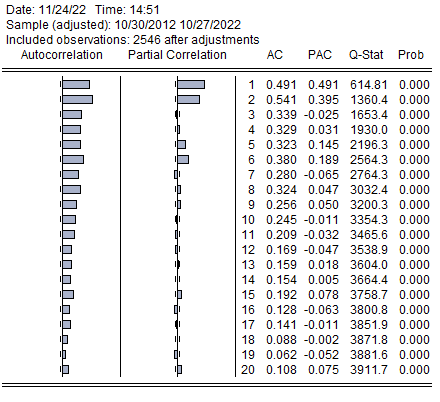
\includegraphics[width=.6\textwidth]{sp500corr_sq}.
\end{center}
Alternatively, we can regress the return on an intercept and inspect the correlogram of the squared residuals (under \texttt{Residual Diagnostics...}).
There is clear evidence of autocorrelation in the squared returns (all $Q$-stats are significant), indicative of the presence of volatility clustering. Since the SPACF seems to more or less drop to zero after 6 lags, we might try an ARCH(6) model. Usually, a simple GARCH(1, 1) will do better though.
\item The ARCH-LM test is only offered after a regression has been estimated, so we start by regressing the returns on an intercept. The test is then available under \texttt{View$\rightarrow$Residual Diagnostics$\rightarrow$Heteroskedasticity Tests}. We choose to include 5 lags (one trading week). The result is shown below.
\begin{center}
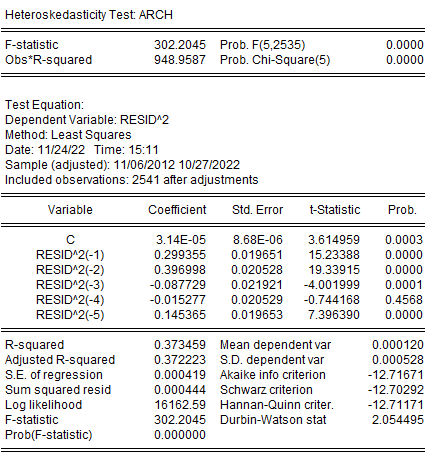
\includegraphics[width=.6\textwidth]{sp500_archlm}
\end{center}
The null of no heteroskedasticity is clearly rejected; the $p$-value is essentially zero, and the test observed test statistic $T\cdot R^2_{aux}$ is much larger than the critical value 11.07.
\item The historical volatility forecasts can be obtained via
\begin{verbatim}
genr sigma_hist(1) = @sqrt(@movav(r^2, 250))
\end{verbatim}
The (1) on the LHS is there because \verb.@movav. includes the observation at time $t$, and we can only include that in our forecast for time $t+1$. Alternatively, if you don't want to assume a zero mean for the daily returns, you can do
\begin{verbatim}
genr sigma_hist2(1) = @movstdevp(r, 250)
\end{verbatim}
Plotting the historical volatility produces the figure below.
\begin{center}
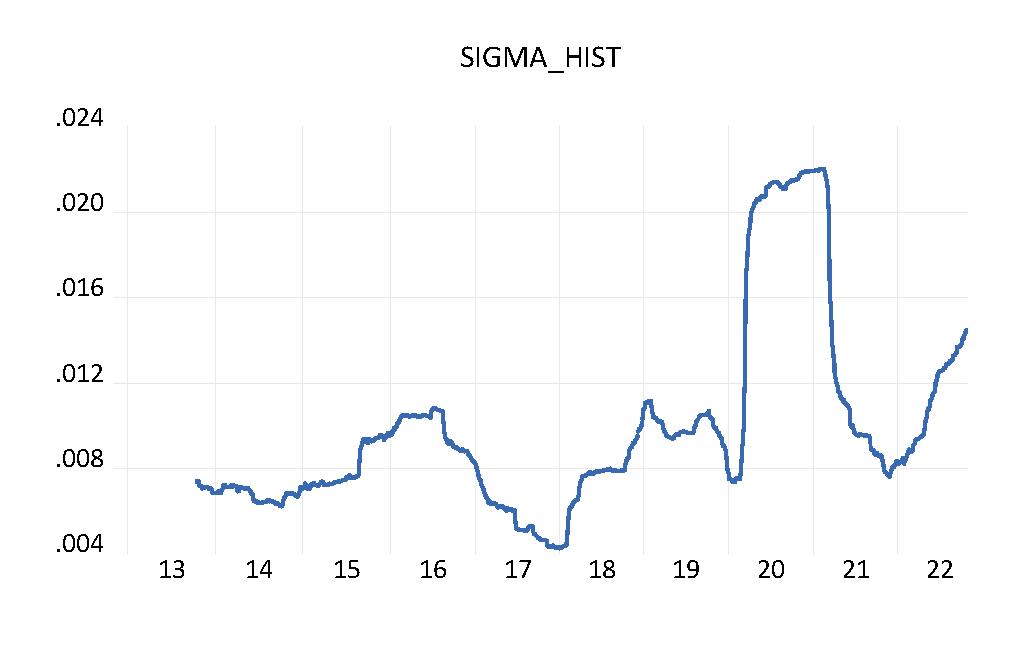
\includegraphics[width=.6\textwidth]{historical}.
\end{center}

\item The RiskMetrics volatility with $\lambda=0.94$ is obtained as follows:
\begin{verbatim}
scalar lambda = .94
smpl @first+2 @first+2
series sigma_EWMA = r(-1)^2
smpl @first+3 @last
sigma_EWMA = lambda * sigma_EWMA(-1) + (1-lambda) * r(-1)^2
sigma_EWMA = @sqrt(sigma_EWMA)
\end{verbatim}
Graphically, it looks as follows.
\begin{center}
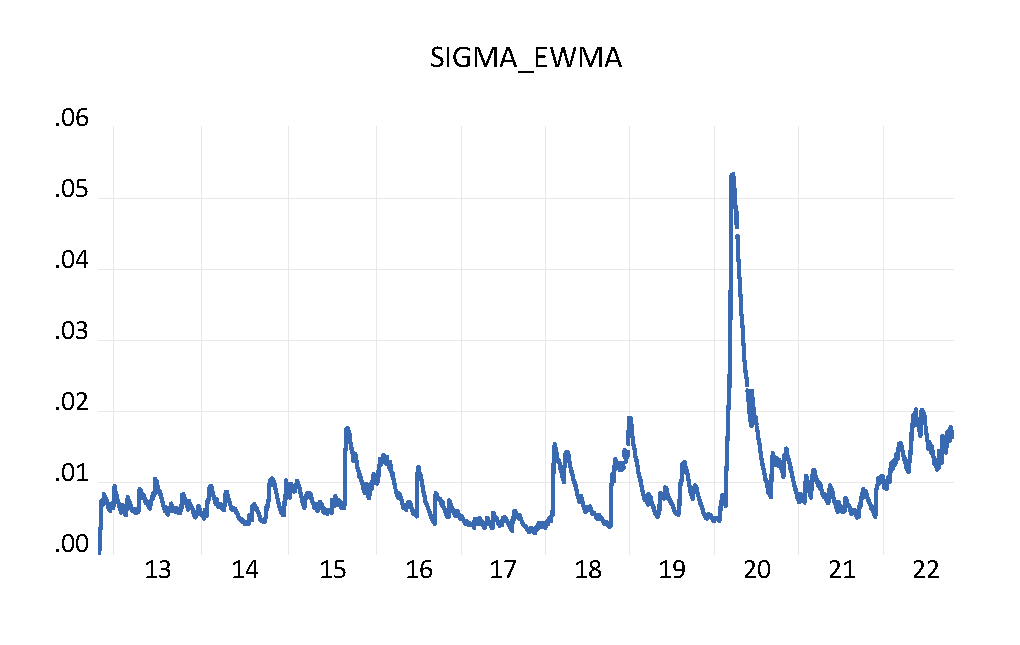
\includegraphics[width=.9\textwidth]{ewma94}
\end{center}
\item ARCH models can be estimated by clicking \texttt{Quick$\rightarrow$Estimate Equation\ldots} and changing the estimation method to ARCH. To fit an ARCH(6), enter the dependent variable at the top, followed by any regressors (this is called the \emph{mean equation}). We only include an intercept, but it's also possible to include ARMA terms if there is any autocorrelation. Then, specify 6 ARCH lags (this is $q$), zero GARCH lags (this is $p$), and a zero threshold order (this is for GJR/TARCH):
\begin{center}
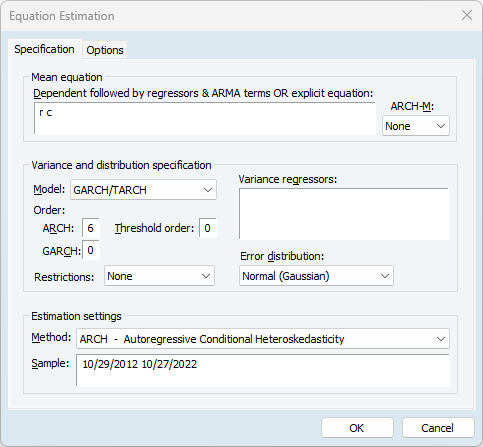
\includegraphics[width=.6\textwidth]{quick}.
\end{center}
You should also select Bollerslev-Wooldridge standard errors in the \texttt{Options} tab, because we will see later that the standardized residuals will not be normally distributed:
\begin{center}
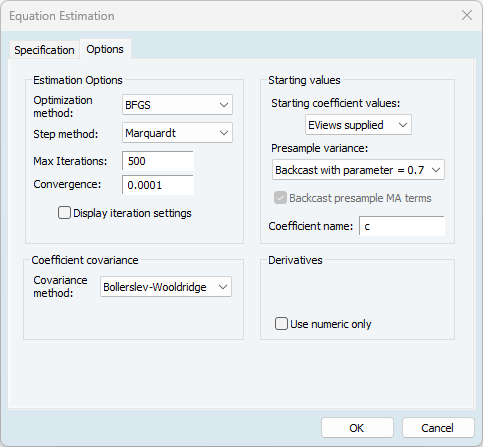
\includegraphics[width=.6\textwidth]{options}.
\end{center}
The estimated model is
\begin{center}
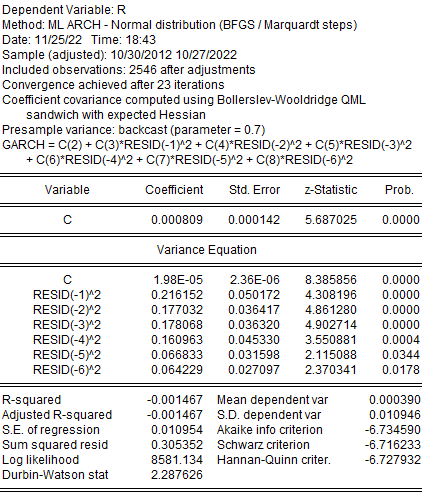
\includegraphics[width=.6\textwidth]{arch6}
\end{center}
To see if the model is adequate, we can look at the correlogram of the squared standardized residuals (under \texttt{View$\rightarrow$Residual Diagnostics$\rightarrow$\linebreak Correlogram Squared Residuals}).  It looks as follows.
\begin{center}
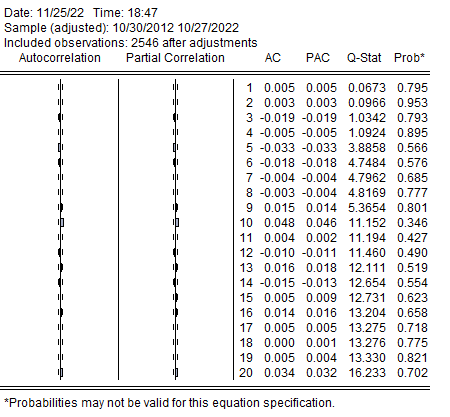
\includegraphics[width=.6\textwidth]{arch6corrsq}
\end{center}
None of the $Q$-tests reject, so there is no remaining autocorrelation.
Alternatively, we can try a GARCH(1, 1) model. This produces
\begin{center}
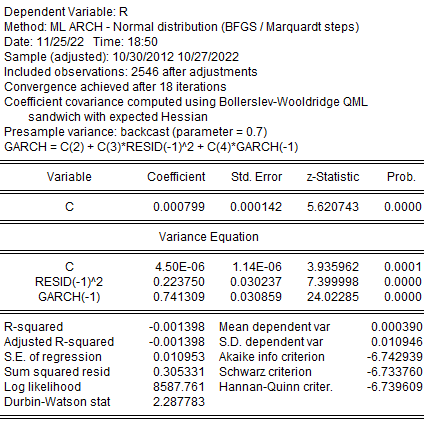
\includegraphics[width=.6\textwidth]{garch11}
\end{center}
The estimated coefficients are $\hat{\beta}=0.74$ and $\hat\alpha=0.22$. This is a bit unusual; typically we find $\hat\beta$ around 0.9 for daily returns (c.f. $\lambda=0.94$ for the RiskMetrics model). The fact that the estimated model is close to the stationarity border (recall that stationarity requires $\alpha+\beta<1$) is typical, though. The correlogram of the squared standardized residuals looks as follows.
\begin{center}
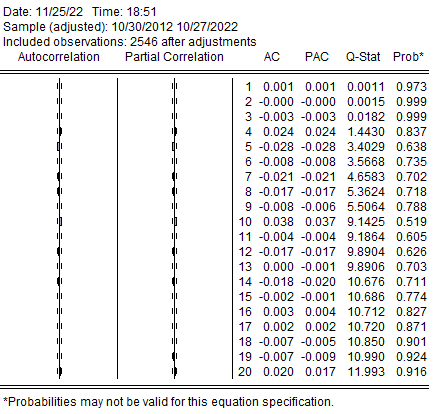
\includegraphics[width=.6\textwidth]{garch11corrsq}
\end{center}
This looks equally good as the ARCH(6). As usual, we prefer smaller models, so we stick with the GARCH(1, 1)\footnote{We could also use the BIC to confirm this decision.}. We can confirm that there is no remaining volatility clustering by running an ARCH-LM test on the standardized residuals   (under \texttt{View$\rightarrow$Residual Diagnostics$\rightarrow$ARCH LM Test}).
\begin{center}
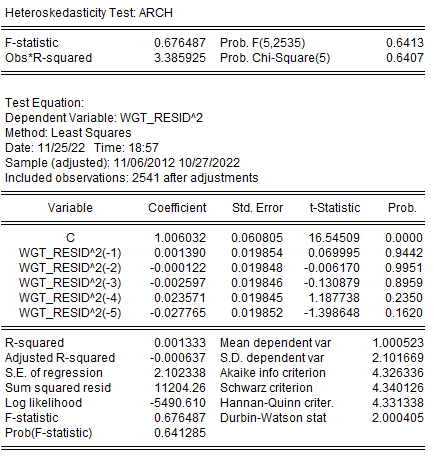
\includegraphics[width=.6\textwidth]{archlmresides}
\end{center}
The test doesn't reject, so it seems that we have successfully modeled the volatility clustering. We can look at a histogram of the standardized residuals by clicking on \texttt{View$\rightarrow$Residual Diagnostics$\rightarrow$Histogram - Normality Test}. This produces the following plot.
\begin{center}
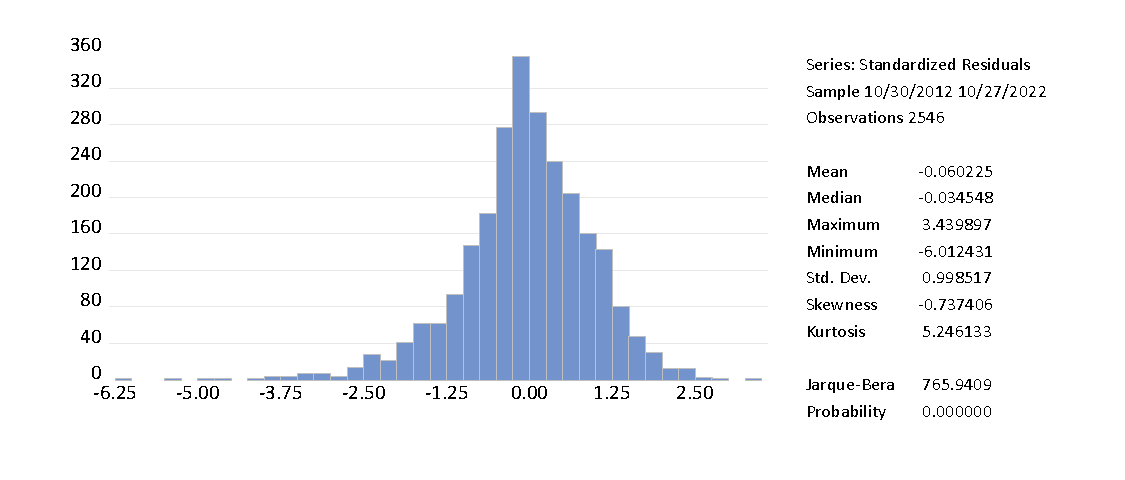
\includegraphics[width=.8\textwidth]{hist}
\end{center}
Normality is clearly rejected, another typical finding. This means that we  were right to use Bollerslev-Wooldridge standard errors. Alternatively, we could have specified a different error distribution, but we'll reserve that for next week.

EViews doesn't offer a statistical test for the leverage effect, so we'll just go ahead and estimate a TARCH(1, 1, 1) model. The fitted model is
\begin{center}
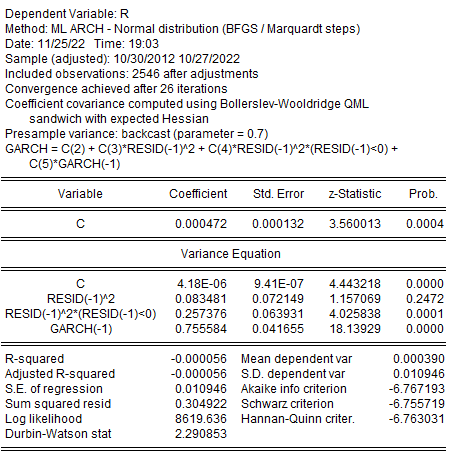
\includegraphics[width=.6\textwidth]{tarch}
\end{center}
The asymmetry coefficient $\hat\gamma=0.257$ is clearly significant, so there is clear evidence of leverage. Also note that the ARCH coefficient has become insignificant. This means that volatility shows no significant reaction to good news (positive returns) at all, only to bad news.
\item The plots can be found under \texttt{View$\rightarrow$GARCH Graphs} and look as follows.
\begin{center}
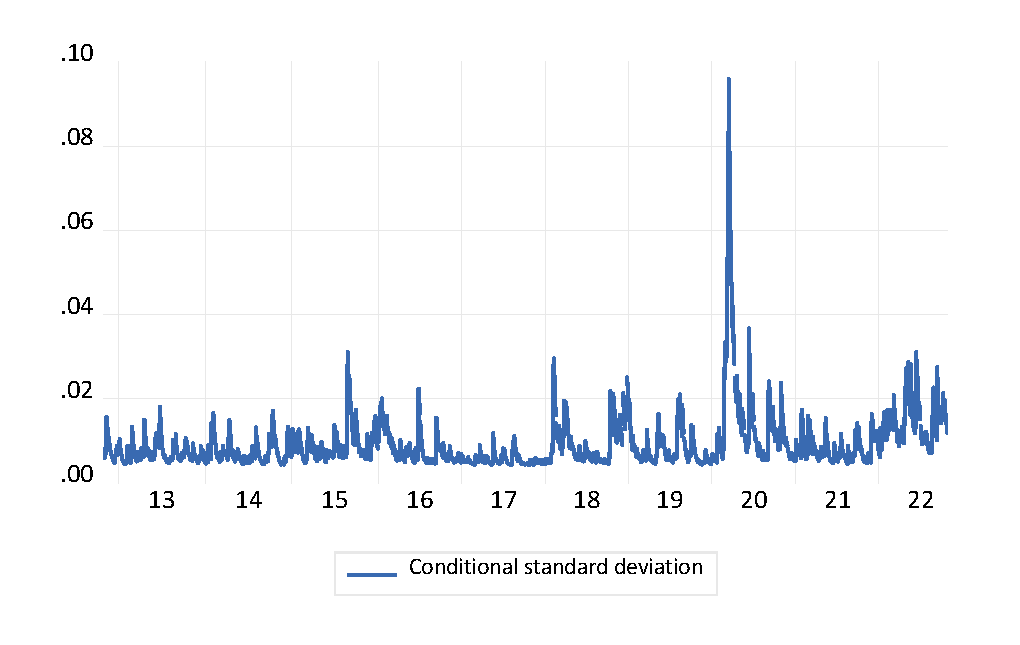
\includegraphics[width=.8\textwidth]{tarch_sigmas}
\end{center}
\begin{center}
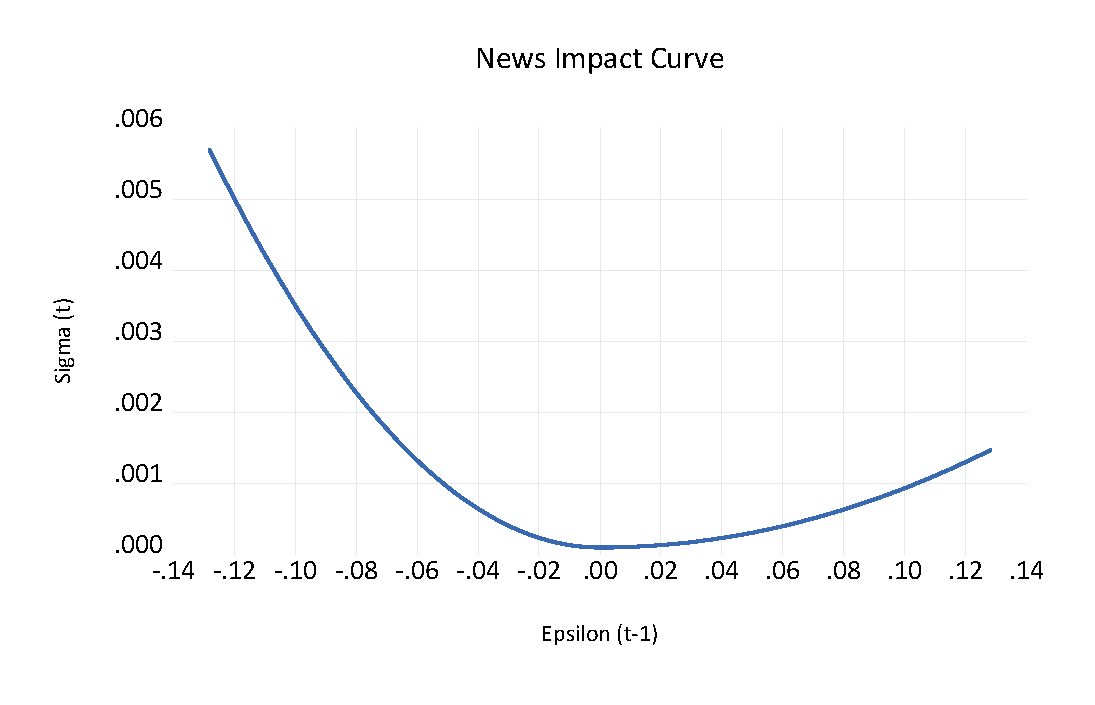
\includegraphics[width=.8\textwidth]{tarch_nic}
\end{center}
\item As usual, we can use EViews for the forecasts, or do it manually. We'll do the latter. To do that, we need the estimated $\widehat{\sigma}_t$ and $\hat{u}_t$. We can get them via \texttt{Proc$\rightarrow$ Make GARCH Variance Series\ldots} and \texttt{Proc$\rightarrow$ Make Residual Series\ldots}. For the latter, you can specify either the ordinary residuals $\hat{u}_t$ or the standardized residuals $\hat{z}_t$. We need the former; the latter would be needed for forecastin and EGARCH model.
    We find that the residual for 27/10 is -0.006573, and the corresponding $\widehat{\sigma}_t$ is 0.0001399. This is all we need to produce a forecast, by plugging into our estimated model as follows.
\begin{align*}
\widehat{\sigma} _{t+1}^{2}&=\hat\omega +\hat\alpha \hat u_{t}^{2}+\hat\gamma \hat u_{t}^{2}\text{I}_{t}+\hat\beta \hat\sigma _{t}^{2}\\
&=0.00000418 +0.083 \hat u_{t}^{2}+0.257 \hat u_{t}^{2}\cdot 1+0.756 \hat\sigma _{t}^{2}\\
&=0.0^5418 +0.083 \cdot(-0.006573)^2+0.257\cdot (-0.006573)^2+0.756 \cdot0.0001399\\&=0.0001246;
\end{align*}
note that the indicator function is 1 because $\hat{u}_t$ is negative.

\end{enumerate}
\item
\begin{enumerate}
\item Splitting out the first term of the sum immediately yields
\begin{align*}
 \widehat{\sigma}_{t+1,EWMA}^{2}  &=(1-\lambda )\sum_{j=0}^{\infty }\lambda ^{j}r_{t-j}^{2} \\
 \widehat{\sigma}_{t+1,EWMA}^{2}  &=(1-\lambda ) \lambda^0 r_{t-0}^2+(1-\lambda )\sum_{j=1}^{\infty }\lambda ^{j}r_{t-j}^{2} \\
 \widehat{\sigma}_{t+1,EWMA}^{2}  &=(1-\lambda ) r_{t}^2+(1-\lambda )\sum_{j=0}^{\infty }\lambda ^{j+1}r_{t-1-j}^{2} \\
 \widehat{\sigma}_{t+1,EWMA}^{2}  &=(1-\lambda ) r_{t}^2+\lambda(1-\lambda )\sum_{j=0}^{\infty }\lambda ^{j}r_{t-1-j}^{2} \\
&=(1-\lambda )r_{t}^{2}+\lambda\widehat{\sigma}_{t,EWMA}^{2}.
\end{align*}
\item Solving $\widehat{\sigma}^2=\hat{\omega} /(1-\hat\alpha -\hat\beta )$ for $\hat{\omega}$, we find $\hat{\omega}=\widehat{\sigma}^2\cdot(1-\hat\alpha -\hat\beta )$. Plugging this into
the equation
\begin{align*}
\widehat{\sigma} _{t+1}^{2}&=\hat{\omega}+\hat{\alpha}\hat{u}_{t}^{2}+\hat{\beta} \widehat{\sigma} _{t}^{2}\\
\intertext{yields}
\widehat{\sigma} _{t+1}^{2}&=\widehat{\sigma}^2\cdot(1-\hat\alpha -\hat\beta )+\hat{\alpha}\hat{u}_{t}^{2}+\hat{\beta} \widehat{\sigma} _{t}^{2}\\
&=\widehat{\sigma}^2+\hat{\alpha}(\hat{u}_{t}^{2}-\widehat{\sigma}^2)+\hat{\beta} (\widehat{\sigma} _{t}^{2}-\widehat{\sigma}^2).
\end{align*}
\item
The result of the previous question also implies that
\begin{align}
\widehat{\sigma} _{t+2}^{2}&=\widehat{\sigma}^2+\hat{\alpha}(\hat{u}_{t+1}^{2}-\widehat{\sigma}^2)+\hat{\beta} (\widehat{\sigma} _{t+1}^{2}-\widehat{\sigma}^2).\notag
\intertext{Replacing the unknown $\hat{u}_{t+1}^{2}$ with its forecast $\widehat{\sigma} _{t+1}^{2}$, we see that}
\widehat{\sigma} _{t+2}^{2}&=\widehat{\sigma}^2+\hat{\alpha}(\widehat{\sigma} _{t+1}^{2}-\widehat{\sigma}^2)+\hat{\beta} (\widehat{\sigma} _{t+1}^{2}-\widehat{\sigma}^2)\notag\\
\widehat{\sigma} _{t+2}^{2}&=\widehat{\sigma} ^{2}+(\hat\alpha+\hat\beta) (\widehat{\sigma}_{t+1}^{2}-\widehat{\sigma} ^{2}).\label{eq1}\\
\intertext{Equation \eqref{eq1} also implies that}
\widehat{\sigma} _{t+3}^{2}&=\widehat{\sigma} ^{2}+(\hat\alpha+\hat\beta) (\widehat{\sigma}_{t+2}^{2}-\widehat{\sigma} ^{2}),\label{eq2}\\
\intertext{and plugging \eqref{eq1} into \eqref{eq2} results in}
\widehat{\sigma} _{t+3}^{2}&=\widehat{\sigma} ^{2}+(\hat\alpha+\hat\beta) ((\hat\alpha+\hat\beta) (\widehat{\sigma}_{t+1}^{2}-\widehat{\sigma} ^{2}))\notag\\
&=\widehat{\sigma} ^{2}+(\hat\alpha+\hat\beta)^2 (\widehat{\sigma}_{t+1}^{2}-\widehat{\sigma} ^{2}).\notag\\
\intertext{Iterating this process produces}
\widehat{\sigma} _{t+s}^{2}&=\widehat{\sigma} ^{2}+(\hat\alpha+\hat\beta)^{s-1} (\widehat{\sigma}_{t+1}^{2}-\widehat{\sigma} ^{2})\notag
\end{align}
as claimed.

\end{enumerate}
\end{enumerate}
\end{document} 